%
% A header that lets you compile a chapter by itself, or inside a larger document.
% Adapted from stackoverflow.com/questions/3655454/conditional-import-in-latex
%
%
%Use \inbpdocument and \outbpdocument in your individual files, in place of \begin{document} and \end{document}. In your main file, put in a \def \ismaindoc {} before including or importing anything.
%
% David Duvenaud
% June 2011
% 
% ======================================
%
%


\ifx\ismaindoc\undefined
	\newcommand{\inbpdocument}{
		\def \ismaindoc {}
		% Use this header if we are compiling by ourselves.
		\documentclass[a4paper,11pt,authoryear,index]{common/PhDThesisPSnPDF}
		
%\usepackage{draftwatermark}
%\SetWatermarkLightness{0.95}

% ******************************************************************************
% ****************************** Custom Margin *********************************

% Add `custommargin' in the document class options to use this section
% Set {innerside margin / outerside margin / topmargin / bottom margin}  and
% other page dimensions

\ifsetMargin
\else
    \RequirePackage[left=37mm,right=30mm,top=35mm,bottom=30mm]{geometry}
    \setFancyHdr % To apply fancy header after geometry package is loaded
\fi


%\chead{Unfinished draft}
%\cfoot{\texttt{Unfinished draft - compiled on \today{} at \currenttime}}

% *****************************************************************************
% ******************* Fonts (like different typewriter fonts etc.)*************

% Add `customfont' in the document class option to use this section

\ifsetFont
\else
    % Set your custom font here and use `customfont' in options. Leave empty to
    % load computer modern font (default LaTeX font).  

    \RequirePackage{libertine} 
\fi

% *****************************************************************************
% *************************** Bibliography  and References ********************

%\usepackage{cleveref} %Referencing without need to explicitly state fig /table

% Add `custombib' in the document class option to use this section
\ifsetBib % True, Bibliography option is chosen in class options
\else % If custom bibliography style chosen then load bibstyle here

   \RequirePackage[square, sort, numbers, authoryear]{natbib} % CustomBib

% If you would like to use biblatex for your reference management, as opposed to the default `natbibpackage` pass the option `custombib` in the document class. Comment out the previous line to make sure you don't load the natbib package. Uncomment the following lines and specify the location of references.bib file

% \RequirePackage[backend=biber, style=numeric-comp, citestyle=numeric, sorting=nty, natbib=true]{biblatex}
% \bibliography{References/references} %Location of references.bib only for biblatex

\fi


% changes the default name `Bibliography` -> `References'
\renewcommand{\bibname}{References}


% *****************************************************************************
% *************** Changing the Visual Style of Chapter Headings ***************
% Uncomment the section below. Requires titlesec package.

%\RequirePackage{titlesec}
%\newcommand{\PreContentTitleFormat}{\titleformat{\chapter}[display]{\scshape\Large}
%{\Large\filleft{\chaptertitlename} \Huge\thechapter}
%{1ex}{}
%[\vspace{1ex}\titlerule]}
%\newcommand{\ContentTitleFormat}{\titleformat{\chapter}[display]{\scshape\huge}
%{\Large\filleft{\chaptertitlename} \Huge\thechapter}{1ex}
%{\titlerule\vspace{1ex}\filright}
%[\vspace{1ex}\titlerule]}
%\newcommand{\PostContentTitleFormat}{\PreContentTitleFormat}
%\PreContentTitleFormat


% *****************************************************************************
% **************************** Custom Packages ********************************
% *****************************************************************************


% ************************* Algorithms and Pseudocode **************************

%\usepackage{algpseudocode} 


% ********************Captions and Hyperreferencing / URL **********************

% Captions: This makes captions of figures use a boldfaced small font. 
%\RequirePackage[small,bf]{caption}

\RequirePackage[labelsep=space,tableposition=top]{caption} 
%\renewcommand{\figurename}{Figure} %to support older versions of captions.sty
\captionsetup{labelsep = colon,belowskip=12pt,aboveskip=4pt}

% ************************ Formatting / Footnote *******************************

%\usepackage[perpage]{footmisc} %Range of footnote options 


% ****************************** Line Numbers **********************************

%\RequirePackage{lineno}
%\linenumbers

% ************************** Graphics and figures *****************************

%\usepackage{rotating}
%\usepackage{wrapfig}
%\usepackage{float}
\usepackage{subfig} %note: subfig must be included after the `caption` package. 


% ********************************* Table **************************************

%\usepackage{longtable}
%\usepackage{multicol}
%\usepackage{multirow}
%\usepackage{tabularx}


% ***************************** Math and SI Units ******************************

\usepackage{amsfonts}
\usepackage{amsmath}
\usepackage{amssymb}
%\usepackage{siunitx} % use this package module for SI units


% ******************************************************************************
% ************************* User Defined Commands ******************************
% ******************************************************************************

% *********** To change the name of Table of Contents / LOF and LOT ************

%\renewcommand{\contentsname}{My Table of Contents}
%\renewcommand{\listfigurename}{List of figures}
%\renewcommand{\listtablename}{List of tables}


% ********************** TOC depth and numbering depth *************************

\setcounter{secnumdepth}{2}
\setcounter{tocdepth}{2}

% ******************************* Nomenclature *********************************

% To change the name of the Nomenclature section, uncomment the following line

%\renewcommand{\nomname}{Symbols}


% ********************************* Appendix ***********************************

% The default value of both \appendixtocname and \appendixpagename is `Appendices'. These names can all be changed via: 

%\renewcommand{\appendixtocname}{List of appendices}
%\renewcommand{\appendixname}{Appndx}

		% All my custom preamble stuff.  Shouldn't overlap with anything in official-preamble




% Paths to figure and table directories.
\newcommand{\symmetryfigsdir}{figures/symmetries}
\newcommand{\topologyfiguresdir}{figures/topology}
\newcommand{\infinitefiguresdir}{figures/infinite}
\newcommand{\grammarfiguresdir}{figures/grammar}
\newcommand{\introfigsdir}{figures/intro}
\newcommand{\gplvmfiguresdir}{figures/gplvm}
\newcommand{\warpedfiguresdir}{figures/warped-mixtures}
\newcommand{\deeplimitsfiguresdir}{figures/deep-limits}
\newcommand{\quadraturefigsdir}{figures/quadrature}
\newcommand{\additivefigsdir}{figures/additive}
\newcommand{\decompfigsdir}{figures/decomp}
\newcommand{\examplefigsdir}{figures/worked-example}

\usepackage{bm}  % for warped mixtures - is this necessary?
\usepackage{booktabs}
\usepackage{tabularx}
\usepackage{multirow}
\usepackage{datetime}
\renewcommand{\tabularxcolumn}[1]{>{\arraybackslash}m{#1}}
\usepackage{relsize}
\usepackage{graphicx}
\usepackage{amsmath,amssymb,textcomp}
\usepackage{nicefrac}
\usepackage{amsthm}
\usepackage{tikz}
\usetikzlibrary{arrows}
\usetikzlibrary{calc}
\usepackage{nth}
\usepackage{rotating}
\usepackage{array}
\usepackage{fp}
\usepackage{cleveref}   % Note: this package sometimes causes the page counter to reset.
\crefname{equation}{equation}{equations}
\crefname{figure}{figure}{figures}
%\usepackage{common/sectsty}

% Controls capitalization of all headers
%\usepackage{stringstrings}
%\usepackage[explicit]{titlesec}
%\newcommand\SentenceCase[1]{%
%  \caselower[e]{#1}%
%  \capitalize[q]{\thestring}%
%}
%\titleformat{\section}
%  {\normalfont\Large\bfseries}{\thesection}{1em}{\SentenceCase{#1}\thestring}


%\titleformat{\section} % The normal, unstarred version
%    {\Large\bfseries}{}{2ex}
%    {\thesection. \MakeSentenceCase{#1}}

%\titleformat{name=\section,numberless} % The starred version; note the `numberless` key
%    {\Large\bfseries}{}{2ex}
%    {\MakeSentenceCase{#1}}

\usepackage[hyperpageref]{backref}
% Setup to show (pages 4 and 9) sort of thing in the bibliography - DD
%\def\foo{\hspace{\fill}\mbox{}\linebreak[0]\hspace*{\fill}}
%\def\foo{\parbox{3cm}{\hfill}
%\def\foo{\parbox{3cm}{\hfill}
%\newcommand\foo[1]{{\raggedleft{\hfill{\mbox{\hfill{#1}}}}}}
\newcommand{\comfyfill}[1]{% = Thorsten Donig's \signed
  \unskip\hspace*{0.1em plus 1fill}
  \nolinebreak[3]%
  \hspace*{\fill}\mbox{#1}
  \parfillskip0pt\par
}
\newcommand\foo[1]{{\comfyfill{\mbox{#1}}}}
%\newcommand\foo[1]{{\mbox{#1}}}
\renewcommand*{\backref}[1]{}
\renewcommand*{\backrefalt}[4]{%
\ifcase #1 %
%
\or
\foo{(page #2)}%
\else
\foo{(pages #2)}%
\fi
}

\usepackage{stringstrings}

%\newcommand{\headercase}{\
%\DeclareFieldFormat{titlecase}{\MakeSentenceCase{#1}}


%% For submission, make all render blank.
%%%%%%%%%%%%%%%%%%%%%%%%%%%%%%%%%%%%%%%%%%%%%%%%%%%%%%%%%%
%%%% EDITING HELPER FUNCTIONS  %%%%%%%%%%%%%%%%%%%%%%%%%%%
%%%%%%%%%%%%%%%%%%%%%%%%%%%%%%%%%%%%%%%%%%%%%%%%%%%%%%%%%%

%% NA: needs attention (rough writing whose correctness needs to be verified)
%% TBD: instructions for how to fix a gap ("Describe the propagation by ...")
%% PROBLEM: bug or missing crucial bit 

%% use \fXXX versions of these macros to put additional explanation into a footnote.  
%% The idea is that we don't want to interrupt the flow of the paper or make it 
%% impossible to read because there are a bunch of comments.

%% NA's (and TBDs, those less crucially) should be written so 
%% that they flow with the text.

\definecolor{WowColor}{rgb}{.75,0,.75}
\definecolor{SubtleColor}{rgb}{0,0,.50}

% inline
\newcommand{\NA}[1]{\textcolor{SubtleColor}{ {\tiny \bf ($\star$)} #1}}
\newcommand{\LATER}[1]{\textcolor{SubtleColor}{ {\tiny \bf ($\dagger$)} #1}}
\newcommand{\TBD}[1]{\textcolor{SubtleColor}{ {\tiny \bf (!)} #1}}
\newcommand{\PROBLEM}[1]{\textcolor{WowColor}{ {\bf (!!)} {\bf #1}}}

% as margin notes

\newcounter{margincounter}
\newcommand{\displaycounter}{{\arabic{margincounter}}}
\newcommand{\incdisplaycounter}{{\stepcounter{margincounter}\arabic{margincounter}}}

\newcommand{\fTBD}[1]{\textcolor{SubtleColor}{$\,^{(\incdisplaycounter)}$}\marginpar{\tiny\textcolor{SubtleColor}{ {\tiny $(\displaycounter)$} #1}}}

\newcommand{\fPROBLEM}[1]{\textcolor{WowColor}{$\,^{((\incdisplaycounter))}$}\marginpar{\tiny\textcolor{WowColor}{ {\bf $\mathbf{((\displaycounter))}$} {\bf #1}}}}

\newcommand{\fLATER}[1]{\textcolor{SubtleColor}{$\,^{(\incdisplaycounter\dagger)}$}\marginpar{\tiny\textcolor{SubtleColor}{ {\tiny $(\displaycounter\dagger)$} #1}}}

%\renewcommand{\LATER}[1]{}
%\renewcommand{\fLATER}[1]{}
%\renewcommand{\TBD}[1]{}
%\renewcommand{\fTBD}[1]{}
%\renewcommand{\PROBLEM}[1]{}
%\renewcommand{\fPROBLEM}[1]{}
%\renewcommand{\NA}[1]{}


% HUMBLE WORDS: shown slightly smaller when in normal text
% Thanks to Christian Steinruecken!

% HUMBLE WORDS: shown slightly smaller when in normal text
% Christian Steinruecken
%
\makeatletter%
%\def\@humbleformat#1{{\fontsize{}{1em}\selectfont #1}}
%\def\@humbleformat#1{\textsmaller{#1}}%
\newlength{\nonHumbleHeight}
\def\@humbleformat#1{{\settoheight{\nonHumbleHeight}{#1}\resizebox{!}{0.94\nonHumbleHeight}{#1}}}%
\def\@idxhumbleformat#1{{\relscale{0.95}{#1}}}%
%\def\@humbleformat#1{{#1}}%
\def\declareHumble#1#2{%
  \expandafter\def\csname #1\endcsname{\@humbleformat{#2}}%
  \expandafter\def\csname s#1\endcsname{{#2}}%
  \expandafter\def\csname idx#1\endcsname{{\@idxhumbleformat{#2}}}%
}%
\def\humble#1{\@humbleformat{#1}}%
\def\idxhumble#1{\@idxhumbleformat{#1}}%
\makeatother%

% Convenient indexing for humble abbreviations
\def\humbleindex#1#2{\index{#1@\idxhumble{#1}}}



% TODO: Clean up duplicates
\declareHumble{ANOVA}{ANOVA}
\declareHumble{ARD}{ARD}
\declareHumble{BIC}{BIC}
\declareHumble{BMC}{BMC}
\declareHumble{bq}{BQ}
\declareHumble{CRP}{CRP}
\declareHumble{dirpro}{DP}
\declareHumble{HDMR}{HDMR}
\declareHumble{GAM}{GAM}
\declareHumble{GEM}{GEM}
\declareHumble{GMM}{GMM}
\declareHumble{gplvm}{GP-LVM}
\declareHumble{gpml}{GPML}
\declareHumble{GPML}{GPML}
\declareHumble{gprn}{GPRN}
\declareHumble{gpt}{GP}
\declareHumble{gp}{GP}
\declareHumble{HKL}{HKL}
\declareHumble{HMC}{HMC}
\declareHumble{ibp}{IBP}
\declareHumble{iGMM}{iGMM}
\declareHumble{iwmm}{iWMM}
\declareHumble{kCP}{CP}
\declareHumble{kCW}{CW}
\declareHumble{kC}{C}
\declareHumble{KDE}{KDE}
\declareHumble{kLin}{Lin}
\declareHumble{KPCA}{KPCA}
\declareHumble{kPer}{Per}
\declareHumble{kPerGen}{ZMPer}
\declareHumble{kRQ}{RQ}
\declareHumble{kSE}{SE}
\declareHumble{kWN}{WN}
\declareHumble{Lin}{Lin}
\declareHumble{LBFGS}{L-BFGS}
\declareHumble{LIBSVM}{LIBSVM}
\declareHumble{MAP}{MAP}
\declareHumble{mcmc}{MCMC}
\declareHumble{MKL}{MKL}
\declareHumble{MLP}{MLP}
\declareHumble{MNIST}{MNIST}
\declareHumble{MSE}{MSE}
\declareHumble{OU}{OU}
\declareHumble{Per}{Per}
\declareHumble{RBF}{RBF}
\declareHumble{RMSE}{RMSE}
\declareHumble{RQ}{RQ}
\declareHumble{SBQ}{SBQ}
\declareHumble{seard}{SE-ARD}
\declareHumble{sefull}{SE-\textnormal{full}}
\declareHumble{SEGP}{SE-GP}
\declareHumble{SE}{SE}
\declareHumble{SNR}{SNR}
\declareHumble{SSANOVA}{SS-ANOVA}
\declareHumble{SVM}{SVM}
\declareHumble{UCI}{UCI}
\declareHumble{UMIST}{UMIST}
\declareHumble{vbgplvm}{VB GP-LVM}

\newcommand{\kSig}{\boldsymbol\sigma}

\def\subexpr{{\cal S}}
\def\baseker{{\cal B}}
\def\numWinners{k}

\def\ie{i.e.\ }
\def\eg{e.g.\ }
\def\etc{etc.\ }
\let\oldemptyset\emptyset
%\let\emptyset 0




% Unify notation between neural-net land and GP-land.
\newcommand{\hphi}{h}
\newcommand{\hPhi}{\vh}
\newcommand{\walpha}{w}
\newcommand{\wboldalpha}{\bw}
\newcommand{\wcapalpha}{\vW}
\newcommand{\lengthscale}{w}

\newcommand{\layerindex}{\ell}



\newcommand{\gpdrawbox}[1]{
\setlength\fboxsep{0pt}
\hspace{-0.15in} 
\fbox{
\includegraphics[width=0.464\columnwidth]{\deeplimitsfiguresdir/deep_draws/deep_gp_sample_layer_#1}
}}



\newcommand{\procedurename}{ABCD}
\newcommand{\genText}[1]{{\sf #1}}



\newcommand{\asdf}{$^{\textnormal{th}}$}

\newcommand{\binarysum}{\sum_{\bf{x} \in \{0,1\}^D}}
\newcommand{\expect}{\mathbb{E}}
\newcommand{\expectargs}[2]{\mathbb{E}_{#1} \left[ {#2} \right]}
\newcommand{\var}{\mathbb{V}}
\newcommand{\varianceargs}[2]{\mathbb{V}_{#1} \left[ {#2} \right]}
\newcommand{\cov}{\operatorname{cov}}
\newcommand{\Cov}{\operatorname{Cov}}
\newcommand{\covargs}[2]{\Cov \left[ {#1}, {#2} \right]}
\newcommand{\variance}{\mathbb{V}}
\newcommand{\vecop}[1]{\operatorname{vec} \left( {#1} \right)}

\newcommand{\covarianceargs}[2]{\Cov_{#1} \left[ {#2} \right]}
\newcommand{\colvec}[2]{\left[ \begin{array}{c} {#1} \\ {#2} \end{array} \right]}
\newcommand{\tbtmat}[4]{\left[ \begin{array}{cc} {#1} & {#2} \\ {#3} & {#4} \end{array} \right]}

\newcommand{\acro}[1]{{\humble{#1}}}
%\newcommand{\vect}[1]{\boldsymbol{#1}}
\newcommand{\vect}[1]{{\bf{#1}}}
\newcommand{\mat}[1]{\mathbf{#1}}
\newcommand{\pderiv}[2]{\frac{\partial #1}{\partial #2}}
\newcommand{\npderiv}[2]{\nicefrac{\partial #1}{\partial #2}}

\newcommand{\pha}{^{\phantom{:}}}

\newcommand{\argmin}{\operatornamewithlimits{argmin}}
\newcommand{\argmax}{\operatornamewithlimits{argmax}}

% The following designed for probabilities with long arguments

\newcommand{\Prob}[2]{P\!\left(\,#1\;\middle\vert\;#2\,\right)}
\newcommand{\ProbF}[3]{P\!\left(\,#1\!=\!#2\;\middle\vert\;#3\,\right)}
\newcommand{\p}[2]{p\!\left(#1\middle\vert#2\right)}
\newcommand{\po}[1]{p\!\left(#1\right)}
\newcommand{\pF}[3]{p\!\left(\,#1\!=\!#2\;\middle\vert\;#3\,\right)} 
\newcommand{\mean}[2]{{m}\!\left(#1\middle\vert#2\right)}



\newcommand{\valpha}{\boldsymbol{\alpha}}
\newcommand{\va}{\vect{a}}
\newcommand{\vA}{\vect{A}}
\newcommand{\vB}{\mat{B}}
\newcommand{\vb}{\vect{b}}
\newcommand{\vC}{\mat{C}}
\newcommand{\vc}{\vect{c}}
\newcommand{\vecf}{\boldsymbol{f}}
\newcommand{\vell}{\vect{\ell}}
\newcommand{\vepsilon}{\boldsymbol{\epsilon}}
\newcommand{\veps}{\boldsymbol{\epsilon}}
\newcommand{\ve}{\boldsymbol{\epsilon}}
\newcommand{\vf}{\vecf}
\newcommand{\vg}{\vect{g}}
\newcommand{\vh}{\vect{h}}
\newcommand{\vI}{\mat{I}}
\newcommand{\vK}{\mat{K}}
\newcommand{\vk}{\vect{k}}
\newcommand{\vL}{\mat{L}}
\newcommand{\vl}{\vect{l}}
\newcommand{\vmu}{{\boldsymbol{\mu}}}
\newcommand{\vone}{\vect{1}}
\newcommand{\vphi}{{\boldsymbol{\phi}}}
\newcommand{\vpi}{{\boldsymbol{\pi}}}
\newcommand{\vq}{\vect{q}}
\newcommand{\vR}{\mat{R}}
\newcommand{\vr}{\vect{r}}
\newcommand{\vsigma}{{\boldsymbol{\sigma}}}
\newcommand{\vSigma}{\mat{\Sigma}}
\newcommand{\vS}{\mat{S}}
\newcommand{\vs}{\vect{s}}
\newcommand{\vtheta}{{\boldsymbol{\theta}}}
\newcommand{\vu}{\vect{u}}
\newcommand{\vV}{\mat{V}}
\newcommand{\vW}{\mat{W}}
\newcommand{\vw}{\vect{w}}
\newcommand{\vX}{\mat{X}}
\newcommand{\vx}{\vect{x}}
\newcommand{\vY}{\mat{Y}}
\newcommand{\vy}{\vect{y}}
\newcommand{\vzero}{\vect{0}}
\newcommand{\vZ}{\mat{Z}}
\newcommand{\vz}{\vect{z}}


% deep gp notation
\newcommand{\netweights}{w}
\newcommand{\vnetweights}{\vw}
\newcommand{\mnetweights}{\vW}
\newcommand{\outweights}{\v}
\newcommand{\voutweights}{\vv}
\newcommand{\moutweights}{\vV}

\newcommand{\unitparams}{\v}
\newcommand{\vunitparams}{\vv}
\newcommand{\munitparams}{\vV}


\newcommand{\He}{\mathcal{H}}
\newcommand{\normx}[2]{\left\|#1\right\|_{#2}}
\newcommand{\Hnorm}[1]{\normx{#1}{\He}}
\newcommand{\mmd}{{\rm MMD}}


\newcommand{\mf}{\bar{\vf}}

%\newcommand{\mf}{\mu} %{\bar{\ell}}
\newcommand{\lf}{f} % Likelihood function
\newcommand{\st}{_\star}

% from simpler log-bq writeup
\newcommand{\lftwo}{{\log \ell}}
\newcommand{\mftwo}{{\bar \ell}}
\newcommand{\loggp}{{\log\acro{GP}}}%| \bX, \vy )}}
\newcommand{\loggpdist}{{\acro{GP}(\lftwo)}}%| \vX, \vy )}}


\newcommand{\inv}{^{{\mathsmaller{-1}}}}
\newcommand{\tohalf}{^{{\mathsmaller{\nicefrac{1}{2}}}}}

\newcommand{\Normal}{\mathcal{N}}
\newcommand{\N}[3]{\mathcal{N}\!\left(#1 \middle| #2,#3\right)}
\newcommand{\Nt}[2]{\mathcal{N}\!\left(#1,#2\right)}
\newcommand{\NT}[2]{\mathcal{N}\!\left(#1,#2\right)}
\newcommand{\GPdist}[3]{\mathcal{GP}\!\left(#1 \, \middle| \, #2, #3 \right)}
\newcommand{\GPdisttwo}[2]{\mathcal{GP}\!\left(\, #1, #2 \right)}
\newcommand{\bN}[3]{\mathcal{N}\big(#1 \middle| #2,#3\big)}
\newcommand{\boldN}[3]{\text{\textbf{\mathcal{N}}}\big(#1;#2,#3\big)}
\newcommand{\ones}[1]{\mat{1}_{#1}}
\newcommand{\eye}[1]{\mat{E}_{#1}}
\newcommand{\tra}{^{\mathsf{T}}}
%\newcommand{\tra}{^{\top}}
%\mathsf{T}
\newcommand{\trace}{\operatorname{tr}}
\newcommand{\shift}{\operatorname{shift}}
\renewcommand{\mod}{\operatorname{mod}}
\newcommand{\deq}{:=}
\newcommand{\oneofk}{\operatorname{one-of-k}}
%\newcommand{\degree}{^\circ}

\newcommand{\GPt}[2]{\mathcal{GP}\!\left(#1,#2\right)}
%\newcommand{\GPt}[2]{\gp\!\left(#1,#2\right)}

\DeclareMathOperator{\tr}{tr}
\DeclareMathOperator{\chol}{chol}
\DeclareMathOperator{\diag}{diag}

\newenvironment{narrow}[2]{%
  \begin{list}{}{%
  \setlength{\topsep}{0pt}%
  \setlength{\leftmargin}{#1}%
  \setlength{\rightmargin}{#2}%
  \setlength{\listparindent}{\parindent}%
  \setlength{\itemindent}{\parindent}%
  \setlength{\parsep}{\parskip}}%
\item[]}{\end{list}}



\newcommand{\dist}{\ \sim\ }
\def\given{\,|\,}

% Table stuff
\newcolumntype{C}[1]{>{\centering\let\newline\\\arraybackslash\hspace{0pt}}m{#1}}
\newcolumntype{L}[1]{>{\raggedright\let\newline\\\arraybackslash\hspace{0pt}}m{#1}}
\newcolumntype{R}[1]{>{\raggedleft\let\newline\\\arraybackslash\hspace{0pt}}m{#1}}

\newcommand{\defeq}{\mathrel{:\mkern-0.25mu=}}

\def\ie{i.e.\ }
\def\eg{e.g.\ }
\def\iid{i.i.d.\ }
%\def\simiid{\sim_{\mbox{\tiny iid}}}
\def\simiid{\overset{\mbox{\tiny iid}}{\sim}}
\def\simind{\overset{\mbox{\tiny \textnormal{ind}}}{\sim}}
\def\eqdist{\stackrel{\mbox{\tiny d}}{=}}
%\newcommand{\distas}[1]{\mathbin{\overset{#1}{\kern \z@ \sim}}}
%TODO: fix this - it worked outside the thesis!
\newcommand{\distas}[1]{\mathbin{\overset{#1}{\sim}}}

\def\Reals{\mathbb{R}}

\def\Uniform{\mbox{\rm Uniform}}
\def\Bernoulli{\mbox{\rm Bernoulli}}
\def\GP{\mathcal{GP}}
\def\GPLVM{\mathcal{GP-LVM}}




% Kernel stuff

\def\iva{\vect{\inputVar}}
\def\ivaone{\inputVar}
\def\inputVar{x}
\def\InputVar{X}
\def\InputSpace{\mathcal{X}}
\def\outputVar{y}
\def\OutputSpace{\mathcal{Y}}
\def\function{f}
\def\kernel{k}
\def\KernelMatrix{K}
\def\SumKernel{\sum}
\def\ProductKernel{\prod}
\def\expression{e}
\def\feat{\vh}

\newcommand{\kerntimes}{ \! \times \!}
\newcommand{\kernplus}{ \, + \,}


% Proof stuff
\theoremstyle{plain}
\newtheorem{theorem}{Theorem}[section]
\newtheorem{lemma}[theorem]{Lemma}
\newtheorem{prop}[theorem]{Proposition}
\newtheorem{proposition}{Proposition}
\newtheorem*{cor}{Corollary}

% For infinite bq
\newcommand{\iv}{\theta}
\newcommand{\viv}{\vtheta}

% For intro chapter
\newcommand{\funcval}{\vf(\vX)}
\newcommand{\testpoint}{{\vx^\star}}

\newcommand{\underwrite}[2]{{\underbrace{#1}_{\textnormal{#2}}}}



% For kernel figures
\newcommand{\fhbig}{2cm}%
\newcommand{\fwbig}{3cm}%
\newcommand{\kernpic}[1]{\includegraphics[height=\fhbig,width=\fwbig]{\grammarfiguresdir/structure_examples/#1}}%
\newcommand{\kernpicr}[1]{\rotatebox{90}{\includegraphics[height=\fwbig,width=\fhbig]{\grammarfiguresdir/structure_examples/#1}}}%
\newcommand{\addkernpic}[1]{{\includegraphics[height=\fhbig,width=\fwbig]{\grammarfiguresdir/additive_multi_d/#1}}}%
\newcommand{\largeplus}{\tabbox{{\Large+}}}%
\newcommand{\largeeq}{\tabbox{{\Large=}}}%
\newcommand{\largetimes}{\tabbox{{\Large$\times$}}}%
\newcommand{\fixedx}{$x$ (with $x' = 1$)}%

% for warped mixtures
\newcommand{\CLAS}{\vz}  %cluster assignments
\newcommand{\CLASi}{z} % individual cluster assignments


		% ************************ Thesis Information & Meta-data **********************

%% The title of the thesis
\title{Automating statistical modelling}

%\texorpdfstring is used for PDF metadata. Usage:
%\texorpdfstring{LaTeX_Version}{PDF Version (non-latex)} eg.,
%\texorpdfstring{$sigma$}{sigma}

%% The full name of the author
\author{James Robert Lloyd}

%% Department (eg. Department of Engineering, Maths, Physics)
%\dept{Department of Engineering}

%% University and Crest
\university{University of Cambridge}
\crest{
\includegraphics[width=0.25\textwidth]{misc/University_Crest}}

%% You can redefine the submission text:
% Default as per the University guidelines: This dissertation is submitted for
% the degree of Doctor of Philosophy
%\renewcommand{\submissiontext}{change the default text here if needed}

%% Full title of the Degree 
\degree{Doctor of Philosophy}
 
%% College affiliation (optional)
\college{Trinity College}

%% Submission date
\degreedate{December 2014} 

%% Meta information
\subject{Machine Learning}
\keywords{{LaTeX} {PhD Thesis} {Engineering} {University of Cambridge} {Machine Learning} {Gaussian processes} {Time Series} {Model checking} {Model criticism} {Aldous--Hoover} {Networks}}



		\begin{document}
	}	
	\newcommand{\outbpdocument}[1]{
		% Fake chapters so references aren't broken
		\label{ch:intro}                
		\label{ch:dummy}
		\label{ch:discussion}
		%\bibliographystyle{common/CUEDthesis}
		\bibliographystyle{plainnat}
		\bibliography{references.bib}
		\end{document}
	}	
\else
	%If we're inside another document, no need to re-start the document.
	\ifx\inbpdocument\undefined
		\newcommand{\inbpdocument}{}
		\newcommand{\outbpdocument}[1]{}
	\fi
\fi

\inbpdocument

\chapter{Introduction}
\label{ch:intro}

This thesis concerns the challenge of drawing inferences from uncertain data.
We take a probabilistic and Bayesian approach throughout  which is a natural extension of drawing logical inferences from certain information~\citep[e.g.][]{Edwin2003-jh}.
To perform probabilistic inference faithfully one must be able to express all of one's prior information about some situation in the form of a probability distribution.
In chapters~\ref{ch:networks}~and~\ref{ch:arrays} we demonstrate how to construct probability distribution that respect symmetry conditions appropriate for data in the form of networks or databases.
In chapters~\ref{ch:construction}~and~\ref{ch:description} we develop expressive probability distributions over functions and demonstrate that they express patterns that can be easily understood by humans.
In chapter~\ref{ch:gefcom} we demonstrate the application of these distributions over functions to a data mining competition.
Finally, chapter~\ref{ch:criticism} considers the problem of criticising a probabilistic model when we have reason to believe that we were either unable to express our prior information probabilistically or perform inference to a sufficient level of accuracy.
We elaborate on these points in the rest of this chapter.

\section{Bayesians and frequentists}

All chapters of this thesis apart from chapters~\ref{ch:criticism}~and~\ref{ch:gefcom} take an entirely (or at least approximately) Bayesian (or more generally probabilistic) approach to statistical inference.
The situations in which it is wise to perform inference in a Bayesian manner as opposed to using a method justified by its frequentist properties is commonly poorly understood.
As a result, many people still talk about a Bayesians versus frequentists debate as if one paradigm could be declared better than the other \TBD{cite \url{http://www.reddit.com/r/statistics/comments/1ye692/a_fervent_defense_of_frequentist_statistics/} \url{http://lesswrong.com/lw/jne/a_fervent_defense_of_frequentist_statistics/} \url{https://news.ycombinator.com/item?id=7263490} Tibshirani}.
I will therefore devote a small amount of space to the justification of Bayesian inference and also discuss its limitations.

How should we perform rational inferences with uncertain information?
A solution to this question is provided by Cox's theorem\fTBD{cite} which derives a calculus of reasoning about the plausability of statements from three simple axioms of rational behaviour.
A version of these axioms are colloquially stated by \citet{Edwin2003-jh} as
\begin{enumerate}
  \item Degrees of plausibility are represented by real numbers
  \item Qualitative correspondence with common sense
  \item Consistency of reasoning
\end{enumerate}
The calculus that one can logically derive from these axioms is isomorphic to probability theory; plausabilities satisfy the sum and product rules that are typically stated as the axioms of probability theory\fTBD{cite e.g. Kolmogorov}.

This result tells us that if we can accurately specify our beliefs as probability distributions then there is only one way to rationally (in the sense of Cox's axioms) update those beliefs in the light of new data \ie by using probability theory (which includes Bayes' rule).
Thus, we are compelled to perform inference using the rules of probability theory when the following three conditions hold
\begin{enumerate}
  \item We are willing to accept Cox's axioms
  \item We can faithfully express our prior beliefs about a problem using probability distributions
  \item Exact probabilistic inference or a sufficiently close approximation is computationally tractable
\end{enumerate}
There are some who have argued against Cox's axioms\fTBD{Cite from Jaynes} but no widely accepted alternatives currently exist.
Conditions 2 and 3 however are often false; in response one may wish to develop or use a method with frequentist guarantees or one could attempt research which makes them true in a larger number of situations\footnotemark{}.
This thesis is concerned with the latter strategy.

\footnotetext{
Or one could attempt to revise statistical theory in such a way as to take account of computational and epistemic limitations.
These lines of enquiry is potentially very fruitful but still in its infancy\TBD{ Cite Jordan and Swedes and others?}.
}

%Chapters~\ref{ch:networks}~and~\ref{ch:arrays} are concerned with the problem of specifying an appropriate mathematical form of probabilistic model based on symmetry arguments.
%Chapters~\ref{ch:construction}~and~\ref{ch:description} are concerned with producing probability distributions over functions that better match our prior beliefs about the types of function we expect to encounter in data.
%Chapters~\ref{ch:gefcom}~and~\ref{ch:criticism} consider problems where we have good reason to believe that at leats one of conditions 2 and 3 do not hold.
%In particular, chapter~\ref{ch:gefcom} applies the techniques of chapter~\ref{ch:construction} to a data mining competition which reveals some areas where improvements can be made.
%Chapter~\ref{ch:criticism} develops new techniques to investigate probabilistic models where we know that we were unable to specify our prior beliefs faithfully.

\section{An introduction to exchangeability and representation theorems}

Suppose one receives a sequence of data $(X_1, X_2, \dots)$ and we wish to specify our beliefs about this data with a probability distribution.
An often reasonable prior assumption is that we do not believe the order of the data contains any information, or rather that any probability distribution encoding our beliefs about this data should be invariant to reorderings of the data.
That is, we may often believe that our data is an exchangeable sequence:
\[
  \label{eq:intro:exch}
  (X_1, X_2, \dots) \eqdist (X_{p(1)}, X_{p(2)}, \dots) \qquad \forall\, p\in\SGinf
\]
where $\eqdist$ denotes equality in distribution, and $\SGinf$ is the set of all permutations of $\Nats$ which permute at most a finite number of elements.

de Finetti's theorem \citep[e.g.][]{Kallenberg:2005} characterises all probability distributions of sequences with this property;  $(X_i)_{i\in\Nats}$ is an exchangeable sequence if and only if there exists a random probability measure $\AHfunction$ such that $\darray_1,\darray_2,\ldots\simiid\AHfunction$.
In other words, observations are conditionally \iid given some random $\AHfunction$.
For the purposes of probabilistic modelling, this implies that our beliefs about exchangeable sequences of data can be expressed in the form of a distribution over probability measures.
A note on terminology: we will refer to de Finetti's theorem and related results as representation theorems. 

In chapter~\ref{ch:networks} we demonstrate that a generalisation of de Finetti's theorem due to Aldous and Hoover can be used to construct probability distributions of networks and arrays where weaker symmetry assumptions are appropriate.
In chapter~\ref{ch:arrays} we use results by Kallenberg to extend the results of Aldous and Hoover to the case of probability dsitributions for general databases.
We also demonstrate how these representation theorems are compatible with other formalisms and assumptions \eg longitudinal / time-varying data or conditional probability distributions.

\section{An introduction to using Gaussian processes to model functions}

There are a great many (and many great) introductions to Gaussian processes in the literature\fTBD{Cite a bunch}.
Rather than repeat them, I will give an intuitive derivation of Gaussian processes starting from linear regression.
Those with an understanding of Gaussian processes may safely skip this section and those interested in further details are directed to the following reference books\fTBD{cite Rasmussed and Williams and maybe Kallenberg as a nice (lol) contrast}.

Let us consider a simple version of Bayesian linear regression.
Suppose we have a data set $D$ consisting of real-valued (input, output) pairs denoted by $D = \{(x_i, y_i) \in \Reals^2 : i = 1,\dots,n\}$.
A simple probabilistic linear regression model of this data could be of the form.
\[
  m &\sim \Normal(0,1) \label{eq:intro:prior_m} \\
  \varepsilon_i &\simiid \Normal(0,\sigma_\varepsilon^2) \\
  y_i &= m x_i + \varepsilon_i
\]
\ie we believe our data will be linearly related by a line passing through the origin.

For this prior belief it is trivial to update our beliefs in the light of data according to the calculus of probability theory upon which we find
\[
  m \given D &\sim \Normal\bigg(\frac{\sum_i x_i y_i}{\sum_i x_i^2 + \sigma_\varepsilon^2}, \frac{\sigma_\varepsilon^2}{\sum_i x_i^2 + \sigma_\varepsilon^2}\bigg) \label{eq:intro:posterior_m} \\
  y_j \given D &\sim \Normal\bigg(\frac{x_j \sum_i x_i y_i}{\sum_i x_i^2 + \sigma_\varepsilon^2}, \frac{x_j^2 \sigma_\varepsilon^2}{\sum_i x_i^2 + \sigma_\varepsilon^2} + \sigma_\varepsilon^2\bigg) \quad \textrm{where } j \notin \{1,\dots,n\}.
\]
The updates of the prior belief for $m$ \eqref{eq:intro:prior_m} into the posterior belief \eqref{eq:intro:posterior_m} is demonstrated visually in figure~\ref{fig:intro:lin_reg}; as more data is observed one's belief about the parameter $m$ becomes more concentrated.

\begin{figure}[ht]
\centering
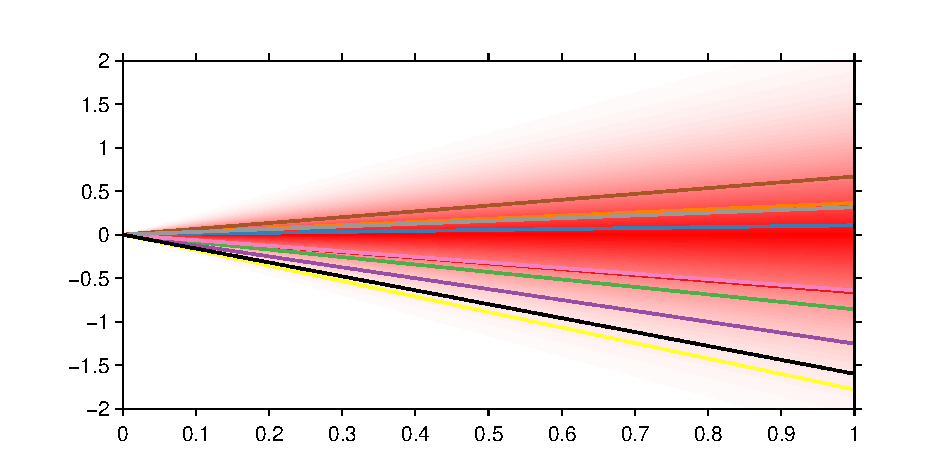
\includegraphics[width=0.3\columnwidth]{\introfigsdir/prior}
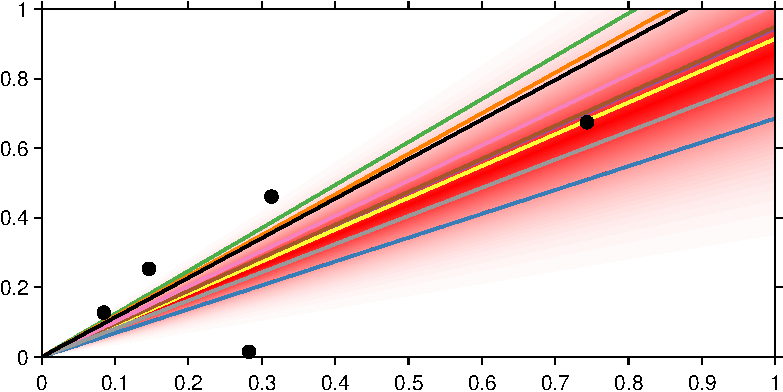
\includegraphics[width=0.3\columnwidth]{\introfigsdir/bayes_5}
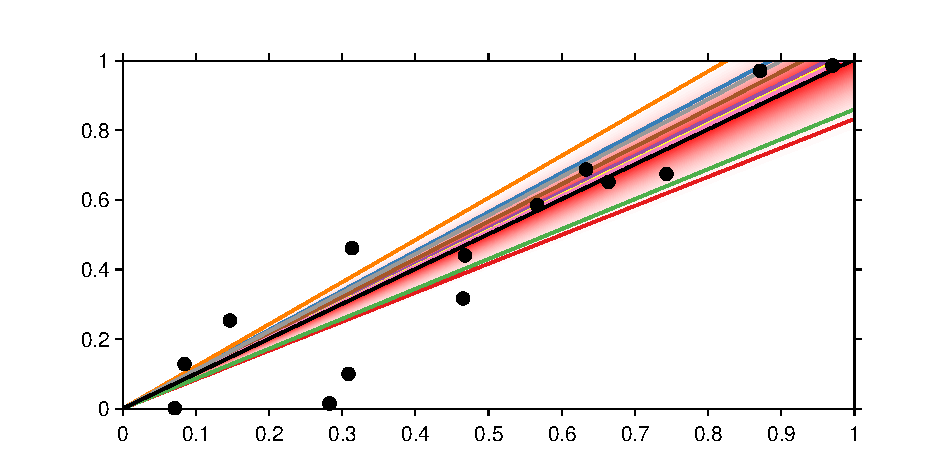
\includegraphics[width=0.3\columnwidth]{\introfigsdir/bayes_15}
\caption{
Bayesian linear regression.
\textit{Left}: Visualisation of prior distribution on gradient $m$.
Lines are random samples from the prior probability distribution, the red shading is a representation of the probability distribution.
\textit{Middle}: Visualiation of the posterior distribution for the gradient $m$ after 5 samples of data have been observed.
\textit{Right}: The posterior after 15 observations.
}
\label{fig:intro:lin_reg}
\end{figure}

We now rewrite the equations for the noisy linear relationship between $y$ and $x$ in an equivalent form
\[
  y_i &\sim \mathcal{N}(0, x_i^2 + \sigma_\varepsilon^2) \\
  \Cov(y_i, y_j) &= x_i x_j \quad \forall\,i\neq j
\]
\ie the prior distribution for $y$ has been assumed to be a multivariate Gaussian distribution
\[
  y \sim \Normal(0, K)
\]
where $K_{ij} = x_i x_j + \delta_{ij} \sigma_\varepsilon^2$ and $\delta_{ij}$ is the Kronecker delta.
Note that we can write this equation for the covariance as a function of pairs of inputs
\[
K_{ij} = k(x_i, x_j) = x_i x_j + \delta_{x_ix_j} \sigma_\varepsilon^2 \label{eq:intro:lin_noise_k}
\]
and this relationship holds for datasets of arbitrary finite size\footnotemark{}.
We now may reasonably ask whether or not we could define a probability distribution over $y$ when $x$ is infinite \eg when $x = \Reals$.
The answer to this question is yes.

\footnotetext{
We are implicitly assuming that the $x_i$ are disjoint.
This can be relaxed without any conceptual difficulty.
}

\begin{definition}[Gaussian process]
  A Gaussian process (\gp{}) is a collection of random variables, any finite subset of which have a joint Gaussian distribution.
\end{definition}

To specify a Gaussian process we must specify the mean and covariance of any finite subset of random variables which we achieve with a mean function $\mu : \mathcal{X} \to \Reals$ and a covariance function or kernel $k : \mathcal{X}^2 \to \Reals$ where $\mathcal{X}$ is the space inhabited by the inputs $x$ which can be written
\[
  y_i &\sim \mathcal{N}(\mu(x_i), k(x_i, x_i)) \\
  \Cov(y_i, y_j) &= k(x_i, x_j)
\]
or alternatively
\[
  (y_i : i = 1,\dots,n) \sim \Normal\bigg(\big(\mu(x_i) : i = 1,\dots,n\big), K\bigg)
\]
where $K_{ij} = k(x_i, x_j)$.
Since these equations hold for any value of the inputs $x$ we can see that by writing $y_i = f(x_i)$ we have essentially specified a probability distribution over functions $f$.
We denote this distribution as
\[
  f \sim \gp(\mu,k).
\]

It is now reasonable to enquire as to the properties of this probability distribution over functions as we change $\mu$ and $k$.
The role of the mean function $\mu$ is particularly easy to characterise; it specifies the pointwise mean of this distribution over functions.
The covariance or kernel $k$ is more interesting.
Random samples from Gaussian processes with a zero mean function but different kernels are shown in figure~\ref{fig:intro:samples}; the randomly sampled functions display qualitatively different patterns of linearity, smoothness and periodicity.

\begin{figure}[ht]
\centering
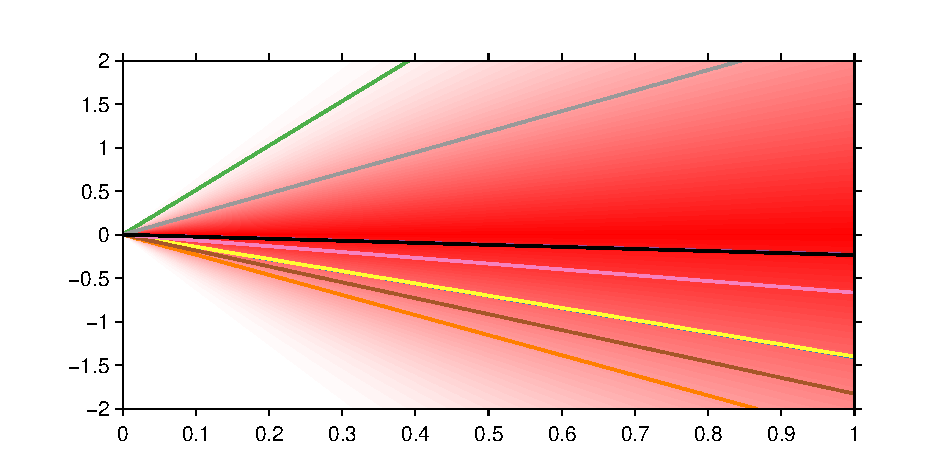
\includegraphics[width=0.3\columnwidth]{\introfigsdir/lin_prior}
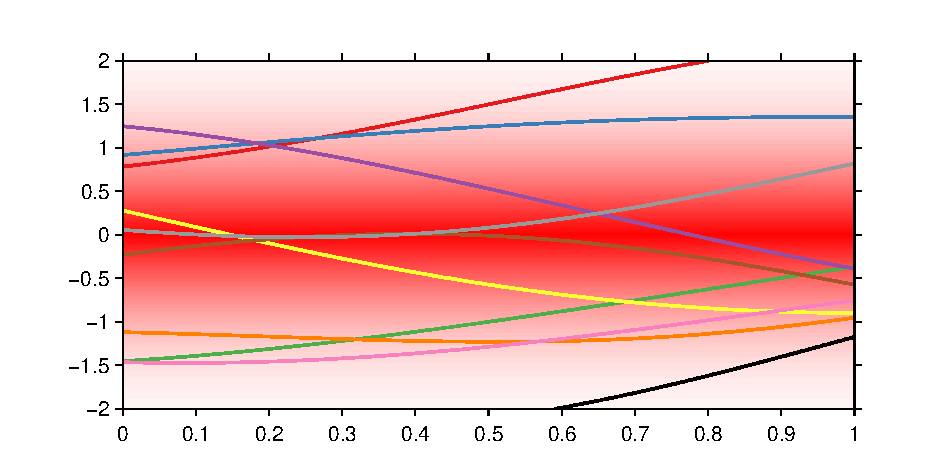
\includegraphics[width=0.3\columnwidth]{\introfigsdir/sq_exp_prior}
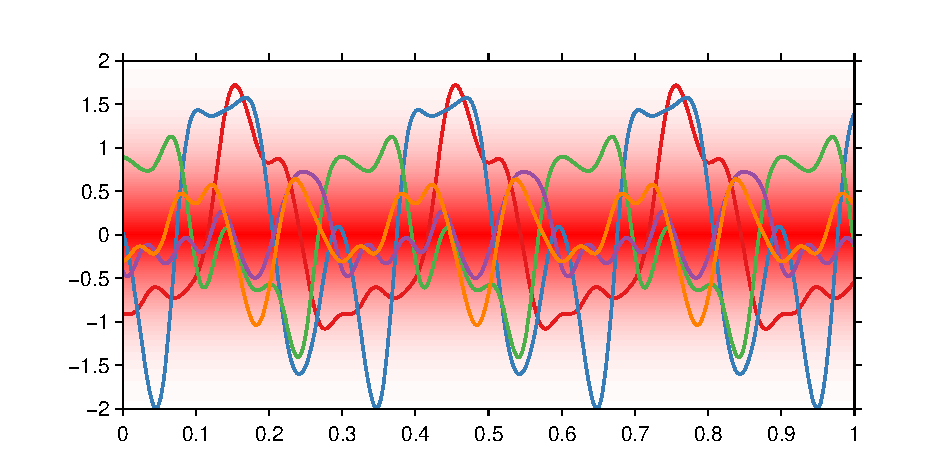
\includegraphics[width=0.3\columnwidth]{\introfigsdir/periodic_prior}
\caption{
Random samples from zero mean Gaussian processes with different covariance functions.
Lines are random samples from the Gaussian process distributions, the red shading is a representation of the pointwise probability distribution.
\textit{Left}: Linear functions.
\textit{Middle}: Smooth and slowly varying functions.
\textit{Right}: Smooth but exactly periodic functions.
}
\label{fig:intro:samples}
\end{figure}

The distribution over linear functions was constructed using a covariance of the form
\[
  k(x_i, x_j) = x_i x_j
\]
which is the same as that in equation~\eqref{eq:intro:lin_noise_k} with the noise variance equal to zero.

The distribution over smooth functions was constructed with a kernel of the form
\[
  k(x_i, x_j) = \exp(-\alpha|x_i - x_j|^2)
\]
where $\alpha$ is a constant.
When the distance between $x_i$ and $x_j$ is small, the covariance (and correlation) between $f(x_i)$ and $f(x_j)$ will be approximately equal to 1.
As a result, nearby values of the function will be similar to each other.
As the distance $|x_i - x_j|$ increases the correlation monotonically decreases to zero; the exact way in which the correlation decreases determines the characteristic smoothness one observes in figure~\ref{fig:intro:samples}.

Finally, the distribution over periodic functions was constructed using a covariance of the form
\[
  k(x_i, x_j) = \exp\left(-\frac{2\sin^2 (\pi(x_i - x_j)/p)}{\ell^2}\right)
\]
where $\ell$ and $p$ are constants.
Whenever $|x_i - x_j|$ is an integer multiple of $p$ the correlation is equal to 1 resulting in exact periodicity of the random functions.

In chapter~\ref{ch:construction} we demonstrate how to learn an appropriate kernel for a particular dataset by constructing new kernels from old.
In chapter~\ref{ch:gefcom} we demonstrate how these ideas were applied to a data mining competition and where this reveals scope for future work.
In chapter~\ref{ch:description} we demonstrate that by carefully choosing which kernels we compose with each other we can always automatically produce natural language descriptions of the probability distributions they encode for.

\outbpdocument{
\bibliographystyle{plainnat}
\bibliography{references.bib}
}


